\chapterimage{/2/head.jpg} % Chapter heading image
\chapter{Universi di Friedmann}\label{2:chuniinfuga}

\section{Equazioni di Friedmann}
I modelli di Friedmann prevedono 3 ingredienti:
\begin{itemize}
    \item Teoria della Relatività Generale (eq. di Einstein)
    \item Universo Omogeneo e Isotropo
    \item Fluido Perfetto
\end{itemize}


Le equazioni di campo di Einstein sono un set di 16 equazioni che descrivono l'interazione gravitazionale come il risultato dell' spazio-tempo curvato da massa ed energia. 
$$R_{\mu \nu} - \frac{1}{2} R \, g_{\mu \nu} = \frac{8 \pi G}{c^4} T_{\mu \nu}.$$

Il membro di sinistra rappresenta la parte geometrica, mediante il tensore di Ricci $R_{\mu \nu}$, il tensore geometrico $g_{\mu \nu}$ e lo scalare di Ricci $R$. Il membro di destra rappresenta il contenuto di energia-materia dell'universo tramite il tensore energia-impulso $T_{\mu \nu}$. 
Nei modelli di Friedmann che prevedono omogeneità e isotropia, il tensore metrico $g_{\mu \nu}$ è descritto dalla metrica di Robertson Walker. Inoltre, assumendo la condizione di fluido perfetto (no viscosità, no conduzione), il tensore energia-impulso dipende esclusivamente da pressione $p$ e densità $\rho$:
$$T_{\mu \nu}=-pg_{\mu \nu}+(p+\rho c^2)u_\mu u_\nu .$$

Delle 16 equazioni soltanto 2 non diventano delle identità e sono quelle tempo-tempo e spazio-spazio:
$$
\ddt{a}=-\frac{4\pi}{3}G\left ( \rho+\frac{3p}{c^2} \right )a\quad (tempo); \qquad
a\ddt{a}+2\dt{a}^2+2kc^2=4\pi G \left ( \rho - \frac{p}{c^2} \right )a^2\quad (spazio).
$$
Ci vorrebbe una settimana di lezioni e calcoli per ottenere tramite la metrica tutti i simboli di Christoffel. Verranno ricavate soltanto in approssimazione newtoniana. In ogni caso, si sostituisce $\ddt{a}$ della prima equazione nella seconda e si ottengono la \textbf{prima e seconda Equazione di Friedmann}.

\begin{align}
   & \dt{a}^2+kc^2  =\frac{8\pi}{3}G\rho a^2 \label{eq:friedmann2}\\
   & \ddt{a}  =-\frac{4\pi}{3}G\left ( \rho+\frac{3p}{c^2} \right )a \label{eq:friedmann1}
\end{align}

Che possono essere legate tra loro dall'equazione di adiabaticità (perché l'universo non dovrebbe essere adiabatico?) nella forma $\mathrm{d}U=-p\mathrm{d}V$ ossia:
\begin{equation}
    \mathrm{d}(\rho c^2 a^3)=-p\mathrm{d}a^3
\end{equation}
Soltanto 2 di queste 3 equazioni sono indipendenti tra di loro.

\vspace{1em}
Proviamo a giustificarle in ambito newtoniano studiando $a$ in funzione del tempo e utilizzando i due teoremi di Birkoff che sono gli equivalenti del teorema di Gauss in relatività generale.
\begin{theorem}[Teoremi di Birkoff]
(1) Il campo gravitazionale di un corpo sferico in uno spazio vuoto è statico ed è descritto al suo esterno dalla metrica di Schwarzschild (quella di un oggetto puntiforme).

(2) Il campo gravitazionale prodotto da un guscio sferico (anche non statico) è descritto al suo interno dalla metrica di Minkowski (quella dello spazio piatto).
\end{theorem}

Si studia la dinamica di un punto $P$ posto su una sfera di raggio $l=d_C \frac{a}{a_0}=:\tilde{D}a$ centrata in $O$. Affinché si possano trascurare gli effetti relativistici, il tempo di collasso libero $\tau_{ff}\propto (G\rho)^{-1/2}$ deve essere molto maggiore del \textit{light crossing time} $\tau =l / c$. Detto in altro modo, si considerano scale più grandi del raggio di Schwarzchild (scala su cui l'energia di massa è in equilibrio con quella gravitazionale). Dall'equazione del moto di Newton, moltiplicata per la derivata nel tempo di $l$, si ha:
$$
\dt{l}\:\frac{\mathrm{d^2} l}{\mathrm{d} t^2}=\frac{Gm}{l^2}\dt{l} \quad \rightarrow \quad \frac{\mathrm{d} }{\mathrm{d} t}\left ( \frac{\dt{l}^2}{2} \right )=\frac{\mathrm{d} }{\mathrm{d} t}\left ( \frac{GM}{l} \right ) \quad \rightarrow \quad \dt{a}^2 =\frac{8\pi}{3}G\rho a^2+cost
$$
Si può ottenere la prima equazione di Friedmann se si assume $cost=-kc^2$. In realtà non è altro che l'equazione di conservazione dell'energia, per la quale $-kc^2$ rappresenta la somma dei contributi di energia cinetica e potenziale. Per $k=0$ si ha un bilanciamente perfetto, per $k=+1$ domina il termine potenziale (collasso) e per $k=-1$ domina il termine cinetico (espansione).

La seconda equazione di Friedmann si ricava in maniera analoga utilizzando un trucchetto relativistico $\rho_{eff}=\rho+3p/c^2$, ossia esiste una densità effettiva data dalla densità di massa e da un termine relativistico legato alla pressione. Si parte comunque dall'equazione di Newton esplicitando la densità e utilizzando la densità effettiva.
Si può dimostrare, per verificare che si è ancora in grado di fare i conti, che utilizzando l'equazione di adiabaticità si riottiene la prima equazione di Friedmann.


In passato l'idea generale era che l'universo dovesse essere statico, ma le relazioni \ref{eq:friedmann1} e \ref{eq:friedmann2} prevedono un universo in espansione. Sarebbe pertanto necessario porre $\rho + 3p/c^2 = 0$, se non fosse che questa condizione è \textit{unphysical} dato che pressione e densità dovrebbero avere un segno discorde. Per cui...
\begin{definition}[Einstein:]
«Grazie mille Sig. Friedmann, ho capito che c'è qualcosa che non va nelle mie equazioni». Senza Fonte.
\end{definition}
... Einstein, nel 1921, introdusse il termine $- \Lambda g_{\mu \nu}$ [L$^2$]:

$$R_{\mu \nu} - \frac{1}{2} R \, g_{\mu \nu} - \Lambda g_{\mu \nu}= \frac{8 \pi G}{c^4} T_{\mu \nu}.$$

Ancora oggi non è chiaro se il termine $- \Lambda g_{\mu \nu}$ sia legato alla geometria dello spazio-tempo come sosteneva Einstein (teoria della gravità modificata) o alla parte energetica (energia oscura, noi votiamo per lei).  
Il tensore energia-impulso viene modificato in: $\tilde{T}_{\mu \nu}=T_{\mu \nu}+\Lambda g_{\mu \nu}\frac{c^4}{8 \pi G}$. Lambda contribuisce in modo negativo alla pressione e positivo alla densità e le equazioni di Friedmann diventano:
\begin{align}
    & \dt{a}^2+kc^2  =\frac{8\pi}{3}G\tilde{\rho} a^2 & \tilde{\rho}=\rho + \rho_\Lambda = \rho + \frac{\Lambda c^2}{8 \pi G} \label{eq:friedmann2tilde} \\
   & \ddt{a}  =-\frac{4\pi}{3}G\left ( \tilde{\rho}+\frac{3\tilde{p}}{c^2} \right )a & \tilde{p}=p + p_\Lambda = p - \frac{\Lambda c^4}{8 \pi G}  \label{eq:friedmann1tilde}
\end{align}


\subsection{Modello di Einstein}
Il modello di Einstein soddisfa le seguenti richieste: 
\begin{itemize}
    \item $\dt{a}=\ddt{a}=0$
    \item Universo di sola materia con $p=p_b=0$
\end{itemize}
Applicando questi vincoli alle equazioni di Friedmann e utilizzando la definizione di $\tilde{p}$ si ha rispettivamente:
$$
\tilde{p} = - \frac{k c^4}{8 \pi G a^2} \quad \mathrm{e}\quad \tilde{p}= -\frac{\Lambda c^4}{8 \pi G} \qquad  \Rightarrow \qquad \Lambda=\frac{k}{a^2}\quad \mathrm{[L^{-2}]}
$$
che mostra come, nel modello di Einstein, $\Lambda$ sia legata al parametro di curvatura. Inoltre si può calcolare qual è la densità ordinaria $\rho$:
$$
\rho = \tilde{\rho} - \rho_\Lambda = \frac{3 k c^2}{8 \pi G a^2} - \frac{k c^2}{8 \pi G a^2}=\frac{k c^2}{4 \pi G a^2}
$$
Questo valore, per avere senso fisicamente, deve essere positivo ossia si deve verificare che $k=+1$.
Infine si può calcolare qual è il valore di $\Lambda$ che rende l'universo statico:
$$
\Lambda_e = \frac{4\pi G\rho}{c^2}
$$
Quindi quello di Einstein è un universo di materia con \textbf{geometria sferica} e diventa statico allorché $\Lambda =\Lambda_e$. 

Per soddisfare il pregiudizio dell'epoca (universo eterno e statico), ha complicato l'equazione in modo arbitrario (pur conservando linearità, ...) e ha dovuto inserire una richiesta cavillosa (la costante cosmologica deve avere un valore ben preciso). Nel 1929 Hubble scoprì l'espansione dell'universo, Einstein prese una penna e scancellò la $\Lambda$ (secondo errore).

\subsection{Modello di De Sitter}
Il modello di De Sitter, seppur stravagante, tornerà utile più avanti per modellare il periodo dell'inflazione. Si basa sulle seguenti assunzioni:
\begin{itemize}
    \item Universo completamente vuoto di materia: $\rho=0$ e $p=0$;
    \item Universo piatto: $k=0$;
    \item L'unico contributo è quello della $\Lambda\neq 0$.
\end{itemize}
Tramite le definizioni di $\tilde{\rho}$ e $\tilde{p} $ si ottiene:
$$
\tilde{p}=-\tilde{\rho}c^2
$$
Si ritroverà questa equazione per la descrizione del vuoto (interpretazione moderna della costante cosmologica). Sostituendo $\rho_\Lambda$ nella prima equazione di Friedmann si ottiene:
\begin{equation}
    a = a_0~e^{H\: t}\qquad H=\frac{\dt{a}}{a}=\sqrt{\frac{\Lambda}{3}}c= cost
\end{equation}
Quindi quello di De Sitter è un universo privo di materia con geometria piatta che evolve con accelerazione esponenziale per un tempo infinito. 

Non esiste un principio fisico che affermi che l'energia del vuoto sia 0. Ogniqualvolta si è trovato un problema nel Modello Standard, la soluzione è stata trovata aggiungendo la costante cosmologica (con un parametro in più i dati fittano meglio). Come negli anni '60 in cui si è scoperto un eccesso di quasar a $z=2$, giustificato da Lemaitre tramite la reintroduzione di $\Lambda$.
\vspace*{0.5em}

\begin{definition}
    The 1960s also saw the discovery of puzzling new astronomical entities, extremely luminous
objects apparently lying at tremendous distance (Schmidt 1963, 1965: Schmidt and Matthews
1964; Sandage 1965). Two unusual aspects of the entities (soon known as quasi-stellar
objects or ‘quasars’) were that they did not appear to conform to the standard relation
between redshift and distance obeyed by ordinary galaxies, while they exhibited a
preponderance of redshifts at around the large value of z = 2 (Hoyle and Burbidge 1966;
Longair and Scheuer 1967; Burbidge and Burbidge 1967). The discovery prompted a new
appraisal of Lemaître’s hesitating model of the cosmos, with a number of
physicists interpreting the phenomenon as evidence for a stagnant phase in cosmic expansion
due to a positive cosmological constant.
Lemaître proposed his famous hypothesis of a universe that originated as a ‘primeval atom’ (Lemaître
1931b; Kragh and Lambert 2007). With such cosmic origins in mind, he noted that a
judicious choice of value for the cosmological constant could give a cosmic expansion in
three stages; an initial phase during which the expansion is de-accelerated by gravity, a
‘loitering’ phase in which the de-acceleration is balanced by the repulsive influence of the
cosmic constant, and a final phase in which the repulsion becomes dominant (Lemaître
1931c, 1931d, 1933). Here the cosmic expansion was governed by a cosmological constant
given $\Lambda=\Lambda_e (1+\varepsilon)$ where the adjustable parameter $\varepsilon$ determined the length of the stagnation period. A schematic of this model, known as the ‘hesitating’ or ‘loitering’ universe is shown below.

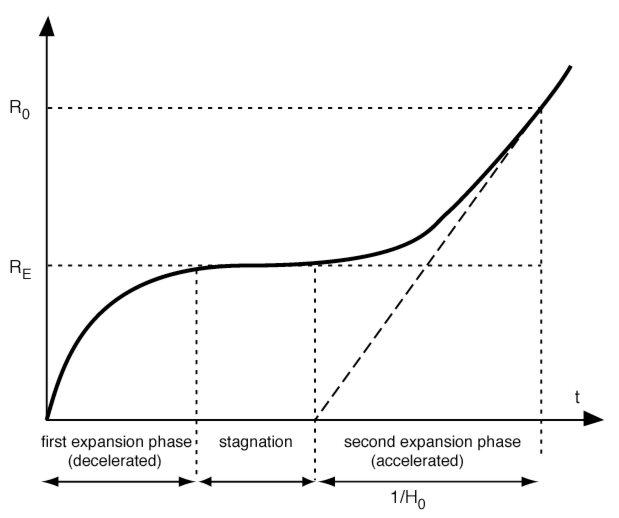
\includegraphics[width=.6\textwidth]{Pictures/2/Uhesitating.png}
\vspace*{0.5em}

From: \cite{oraifeartaigh_one_2018}
\end{definition}
\vspace*{0.5em}
In seguito, si è scoperto che avere così tanti quasar a $z=2$ era dovuto a bias di selezione e la costante cosmologica è stata nuovamente messa da parte. Infine negli anni '70 si è osservato tramite le SNe che l'espansione dell'universo oggi è accelerata e ciò è giustificabile con una costante cosmologica che rende $\ddt{a}>0$ (contribuendo negativamente alla pressione).

\newpage
\section{Soluzioni analitiche del Modello di Friedmann}
Verranno ora discusse più in dettaglio le equazioni di Friedmann per iniziare a descrivere l'attuale Modello Standard.
\subsection{Parametro di densità e geometria}
Manipolando le equazioni di Friedmann è possibile introdurre numerosi parametri strategici per studiare i legami tra le variabili fondamentali della cosmologia.
\begin{align*}
    & \dt{a}^2+kc^2  =\frac{8\pi}{3}G{\rho} a^2 &  H:=\frac{\dt{a}}{\dt{a}} \\
    & \ddt{a}  =-\frac{4\pi}{3}G\left ( {\rho}+\frac{3{p}}{c^2} \right )a   & q:= - \frac{\ddt{a}a}{\dt{a}^2} \\
   & \mathrm{d}(\rho c^2 a^3)= - p \mathrm{d}a^3 & \rho_{cr}:=\frac{3H^2}{8 \pi G}
\end{align*}

Dividendo per $a_0^2$ la prima equazione di Friedmann calcolata ad oggi e utilizzando le definizioni di $H_0$ e $\rho_{\mathrm{cr},0}$, si ottiene:
\begin{equation}
    H_0^2 \left ( 1-\frac{\rho_0}{\rho_{\mathrm{cr},0}}  \right ) = -\frac{kc^2}{a_0^2} \label{eq:friedmannh0rho0}
\end{equation}

Il segno di $k$ è determinato dall'anti-segno della parentesi tonda. Si definisce \textbf{parametro di densità} il valore:
\begin{equation}
    \Omega=\frac{\rho}{\rho_{cr}}\qquad\quad \OmegaO \left\{\begin{matrix}
=1 & \rho_0=\rho_{\mathrm{cr},0} & k=0 & piatto\\ 
>1 & \rho_0>\rho_{\mathrm{cr},0} & k=+1 & sferico\\ 
<1 & \rho_0<\rho_{\mathrm{cr},0} & k=-1 & iperbolico
\end{matrix}\right.
\end{equation}
Affinché l'universo sia piatto e non curvo, il parametro di densità deve avere un valore estremamente preciso (per questo motivo è detta densità \textit{critica}).
Il suo valore attuale (\cite{collaboration2018planck}) vale\footnote{Per accomodare le incertezze, la costante di Hubble viene convenzionalmente scritta: $H_0 = 100\: h$ km s$^{-1}$ Mpc$^{-1}$, una buona approssimazione è $h=0.7$.}:
\begin{align}
    \rho_{\mathrm{cr},0} & \simeq 1.9\:h^2 \cdot 10^{-29}\quad [\mathrm{g\;cm^{-3}}] \\
    & \simeq 2.8\: h^2\cdot 10^{11}\quad [\mathrm{M_\odot\;Mpc^{-3}}]
\end{align}
che è molto simile al valore $\rho_0$ misurato, quindi il nostro universo è spazialmente piatto.

Nel calcolo della densità vanno considerate tutte le componenti.
Nell'universo attuale materia ed energia oscura dominano, possiamo descrivere l'universo come un fluido costituito da due componenti. Per far ciò si utilizzano le definizioni di $\tilde{\rho}$ e $\tilde{p}$ nella seconda equazione di Friedmann:
$$
\ddt{a}  =-\frac{4\pi}{3}G\left ( \rho+\frac{3p}{c^2} \right ) a + \frac{\Lambda c^2}{3}a
$$
Grazie al secondo termine \textbf{si potrebbe avere un'accelerazione positiva}.
Dividendo l'altra equazione per $a_0^2$ si ha:
\begin{equation}
    H_0^2 \left ( 1-\frac{\rho_0}{\rho_{\mathrm{cr},0}} -\frac{\rho_{\Lambda 0}}{\rho_{\mathrm{cr},0}} \right ) = -\frac{kc^2}{a_0^2}
\end{equation}
da cui introducendo il parametro di densità totale:
\begin{equation}
    H_0^2 \left ( 1-\OmegaTOT \right ) = -\frac{kc^2}{a_0^2}\qquad \OmegaTOT=\OmegaO+\OmegaLo \label{eq:2omega0k}
\end{equation}
La curvatura è ora definita da quanto la somma delle due componenti differisce dall'unità (ocio: $\OmegaO = \Omegamo$ ossia in questo caso $\OmegaO$ è riferito alla materia). 


\subsection{Equazione di stato}
L'Universo è costituito da 3 principali componenti:

\begin{example}[Materia non relativistica]
$p_m=nk_B T = \rho_mk_B T/{m_p} \approx 0 \qquad ( \rho_m \approx 0) $
\end{example}
\begin{example}[Radiazione o Materia relativistica]
$p_r=\rho_r c^2/3 $
\end{example}
\begin{example}[Costante Cosmologica]
$p_\Lambda= -\rho_\Lambda c^2 $
\end{example}

In cosmologia si definisce quindi il termine $w$ per l'equazione di stato:
\begin{equation}
    p=w\rho c^2\quad\rightarrow \quad c_s^2=\left ( \frac{\partial p}{\partial \rho}\right )_{S}=wc^2 \qquad \quad w= \left\{\begin{matrix}
0& materia\\
1/3 & radiazione\\
-1 & cost. cosm.
\end{matrix}\right.
\end{equation}
Affinché la velocità del suono $c_s$ rimanga minore di quella della luce $c$, bisogna che $w<1 $ (a $w=1 $ si ha quella conosciuta come \textit{stiff matter}). Inoltre, la non negatività della pressione nella fisica ordinaria richiede $w\geq 0 $. Quindi il \textbf{parametro dell'equazione di stato} $w $ nella fisica ordinaria può assumere un valore $0\leq w\leq 1$ (\textit{intervallo di Zeldovich}).

Armati di tutto questo, lo si applica all'equazione di adiabaticità, si sviluppa il differenziale e si integra per separazione di variabili, ottenendo:
\begin{equation}
    \rho=\rho_0 \left ( \frac{a}{a_0}\right )^{-3(1+w)}\qquad\rightarrow \qquad \rho \propto z^\alpha \qquad \alpha =
\left\{\begin{matrix}
3 & materia\\
4 & radiazione\\
0 & cost. cosm.
\end{matrix}\right.
\label{eq:rhoaw} \end{equation}
Gli esponenti non ci sorprendono: $a^{-3}$ nel caso della materia è come dire Vol$^{-1}$, nel caso della componente relativistica si aggiunge un altro $a^{-1}$ dovuto al redshift. Gli andamenti con le dovute normalizzazioni sono mostrati in Figura \ref{fig:2rhored}.

\begin{figure}[h]
    \centering
    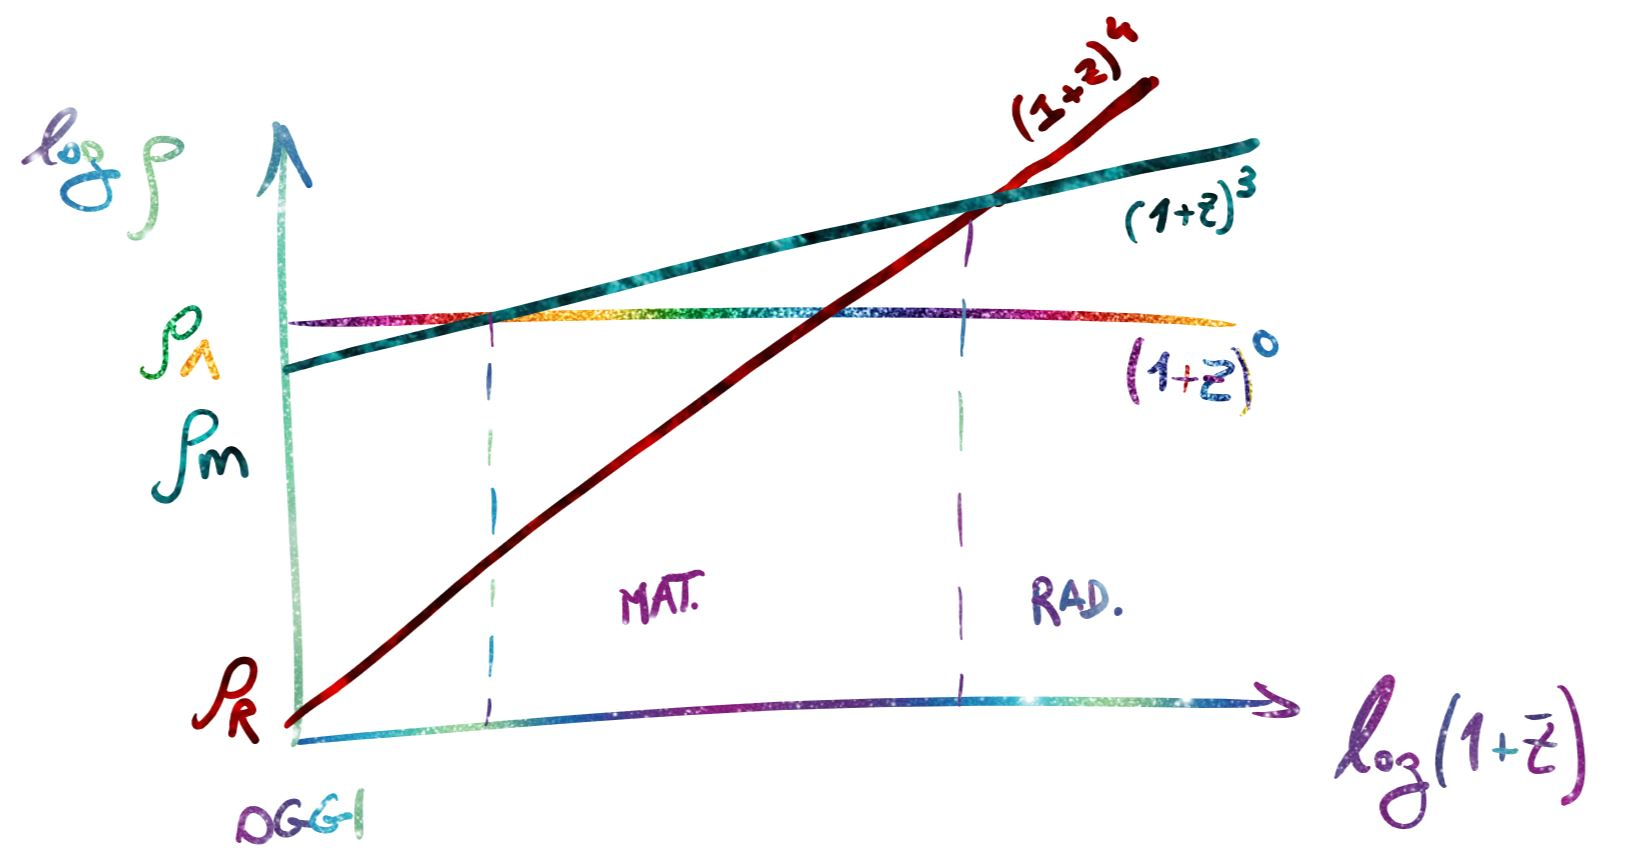
\includegraphics[width=.8\textwidth]{Pictures/2/logrho-z.jpg}
    \caption{Andamento della densità delle tre componenti al variare del redshift.}
    \label{fig:2rhored}
\end{figure}
Sostituendo la (\ref{eq:rhoaw}) nella prima equazione di Friedmann e facendo qualche operazione cosmatematica si ottiene:
\begin{equation}
    H^2=H_0^2\,(1+z)^2\left [ 1-\OmegaO + \OmegaO \,(1+z)^{1+3w} \right ] \label{eq:hevol}
\end{equation}
che regola l'evoluzione del tempo del parametro di Hubble (la geometria è in $\OmegaO$). In universo con più componenti assume la forma generale:
\begin{equation}
    H^2=H_0^2\,(1+z)^2\left [ 1-\sum_{i}\Omega_{i\: 0} + \sum_{i}\Omega_{i\: 0} \,(1+z)^{1+3w_i} \right ] =: H_0^2\; E(z)^2 \label{eq:hevolmulti}
\end{equation}
 

Si assume ora che ci sia una sola componente che rispetti la fisica ordinaria, ossia avente $0\leq w \leq 1$ (e.g. materia). Dalla seconda equazione di Friedmann, $\ddt{a}$ deve essere necessariamente strettamente negativo: la funzione $a(t)$ ha la concavità verso il basso e non può avere un flesso. Inoltre sappiamo osservativamente che l'universo è in espansione $\dt{a}_0>0$. La funzione $a(t)$ è quindi monotona crescente e tornando indietro nel tempo si ha che inevitabilmente interseca l'asse del tempo, ossia deve esistere un $t=0$ (un inizio del tempo, ``Big Bang''). Solo se esistesse un fluido avente $w<-1/3$ si potrebbe avere un flesso.  Il Big Bang è accompagnato da condizioni fisiche antipatiche, ossia per $t\rightarrow 0$ si avrebbe: $a\rightarrow 0$, $\rho \rightarrow \infty$, $T \rightarrow \infty$. Questo è dovuto al fatto che si entra in regimi di cui non si conoscono le leggi fisiche, il limite di validità è il Tempo di Planck $t_P \approx 10^{-43}$ s. Si può evitare il Big Bang con: omogeneità e isotropia violate (metrica non RW), un fluido non perfetto o una componente con $w<-1/3$ (c'è, ma da sola non è sufficiente).

\subsection{Modello di Einstein - De Sitter (EdS)}\label{6:chsub:eds}
Gli universi Einstein - De Sitter sono piatti ($k=0$, $\OmegaO =1$). Le soluzioni sono estremamente importanti perché valgono per buona parte della storia del nostro universo. Partendo dall'equazione (\ref{eq:hevol}) si ottengono le seguenti relazioni:
\begin{equation}\left\{
    \def\arraystretch{2}
        \begin{array}{ll}
            a(t) = a_0 \left ( \frac{t}{t_0} \right )^{\frac{2}{3(1+w)}} \\
            t = t_0 \left ( 1+z \right )^{-\frac{3(1+w)}{2}} \\
            H = \frac{2}{3(1+w)}\frac{1}{t}=\frac{H_0 ~t_0}{t}=H_0 (1+z)^{\frac{3(1+w)}{2}} \\
            q = \frac{1+3w}{2} > 0 \\
            t_0 = \frac{2}{3(1+w)}\frac{1}{H_0} \\
            \rho  = \rho_0 \left ( \frac{t}{t_0} \right )^{-2}= \rho_0 \left(6\pi G (1+w)^2\: t^2\right)^{-1}
    \end{array}\right. \label{eq:modelloeds}
\end{equation}
L'universo è in espansione monotona crescente (ma decelerata in modo costante) ed è infinito. Verso il Big Bang $H\rightarrow \infty$, inoltre all'aumentare di $w$ (pressione) $\ddt{a}$ diventa più basso, fenomeno contrario al concetto di ``scoppio''! Infatti il nome ``Big Bang'' era stato assegnato al modello da coloro che lo sfottevano. Il tempo dell'universo oggi (età) non è esattamente $1/H_0$ per l'effetto della decelerazione dell'espansione.


\begin{table}[h]
\centering
\def\arraystretch{1.5}
\begin{tabular}{@{}ll@{}}
\toprule
\textbf{$w=0$ (materia)} & \textbf{$w=\frac{1}{3}$ (radiazione)} \\ \midrule
$a\propto t^{2/3}$ & $a\propto t^{1/2}$ \\
$t = t_0 \left ( 1+z \right )^{-3/2}$ & $t = t_0 \left ( 1+z \right )^{-2}$ \\
$H = H_0 (1+z)^{3/2} = \frac{2}{3t} $ & $H = H_0 (1+z)^{2} = \frac{1}{2t}$ \\
$q =1/2 $ & $q = 1$ \\
$t_0 = \frac{2}{3}\frac{1}{H_0}$ & $t_0 = \frac{1}{2}\frac{1}{H_0}$ \\
$\rho  = \rho_0\, \frac{1}{6\pi G}\frac{1}{t^2}$ & $\rho  =  \rho_0\, \frac{3}{32\pi G}\frac{1}{t^2}$ \\ \bottomrule
\end{tabular}
\end{table}

\subsection{Universi curvi}
Per analizzare il comportamento dei principali parametri cosmologici nel caso di universi non piatti, si modifica l'equazione (\ref{eq:hevol}) come segue:
$$
\left ( \frac{\dt{a}}{a_0} \right )^2 = H_0^2 \left [ (1-\OmegaO ) + \OmegaO \left ( \frac{a_0}{a} \right )^{1+3w} \right ]
$$
Il primo termine nella parentesi quadra, il termine di curvatura, è costante. Il secondo dipende dal tempo, quindi si studia per quale valore di $a$ i due si equivalgono:
$$
a^*:\quad \left | 1-\OmegaO  \right | = \OmegaO\left ( \frac{a_0}{a^*} \right )^{1+3w}\qquad \leftrightarrow \qquad z^*:\quad \left | \OmegaO^{-1} - 1  \right |^{\frac{1}{1+3w}}
$$

Quando $a\ll a^*$ oppure $z\gg z^*$ (vicino al Big Bang), l'equazione diventa:
$$
\dt{a}=a_0~ H_0 ~\OmegaO^{1/2} \left ( \frac{a_0}{a}\right )^{\frac{1+3w}{2}}
$$
un fattore costante $\OmegaO^{1/2}$ in più rispetto al modello EdS, ossia tutti gli universi curvi si comportano come quello piatto vicino al Big Bang. Un'eventuale curvatura diventerebbe significativa quando  $\left |  1+z^* \right | =  \left | \OmegaO^{-1} - 1  \right |$, ossia a $z< \OmegaO^{-1}$. Per esempio, $z^* =10$ per $\OmegaO=0.1$ e $z^* = 3$ per $\OmegaO=0.3$.

\begin{theorem}[Messaggio da portare a casa]
Anche se fosse curvo, possiamo assumere l'universo piatto per buona parte della sua storia (volendo essere tranquilli sicuramente fino a $z\approx 10$, ma anche a $z\approx 1\div 2$). Per studiare l'eventuale curvatura è necessario fare osservazioni vicine a oggi.
\end{theorem}

Quando $a\gg a^*$ oppure $z\ll z^*$, si può ignorare il termine di curvatura e si distinguono i comportamenti per i due tipi di universo:

\subsubsection{Universi Aperti}
In questo caso $\OmegaO < 1$, quindi $\dt{a}$ è strettamente positiva. Dato che osservativamente $\dt{a}_0 >0$, l'espansione è monotona crescente e vale:
\begin{align}
   & \dt{a}=a_0~ H_0 ~ \sqrt{1-\OmegaO }=cost \\
   & a=a_0~ H_0 ~ \sqrt{1-\OmegaO }~ t  \propto t \\
   & H= 1/t \\
   & q= 0 \\
   & \rho =\rho_{cr} ~\OmegaO \left ( H_0  ~(1-\OmegaO)^{1/2} ~ t   \right )^{-3(1+w)}
\end{align}
In particolare si ha un'espansione lineare libera (non decelerata con nel modello EdS, quindi $a$ negli universi aperti cresce più velocemente). 

\subsubsection{Universi Chiusi}
In questo caso $\OmegaO > 1$, quindi può esistere un valore di $a$ per cui $\dt{a}$ si annulla (si ricorda che dalle osservazioni si ha $\dt{a}_0>0$), ossia la crescita dell'universo si arresta. In particolare questo succede per (si utilizza l'equazione completa):
$$
\dt{a}=0 \quad \rightarrow \quad a_{max}=a_0 \left ( \frac{\OmegaO}{\OmegaO -1} \right )^{\frac{1}{1+3w}}; \quad \rho_{min}=\rho_0 \left ( \frac{\OmegaO -1}{\OmegaO} \right )^{\frac{3(1+w)}{1+3w}}
$$
Questo modello prevede un'espansione fino ad $a_{max}$ e una contrazione con andamento simmetrico (Big Crunch). Per motivi di \textit{quantum cosmology} si potrebbe evitare il completo collasso, generando così quelli conosciuti come universi pulsanti. 

Come sommario si illustrano nella Figura \ref{fig:2at} le tre soluzioni previste per un universo di Friedmann a una sola componente.
\begin{figure}[H]
    \centering
    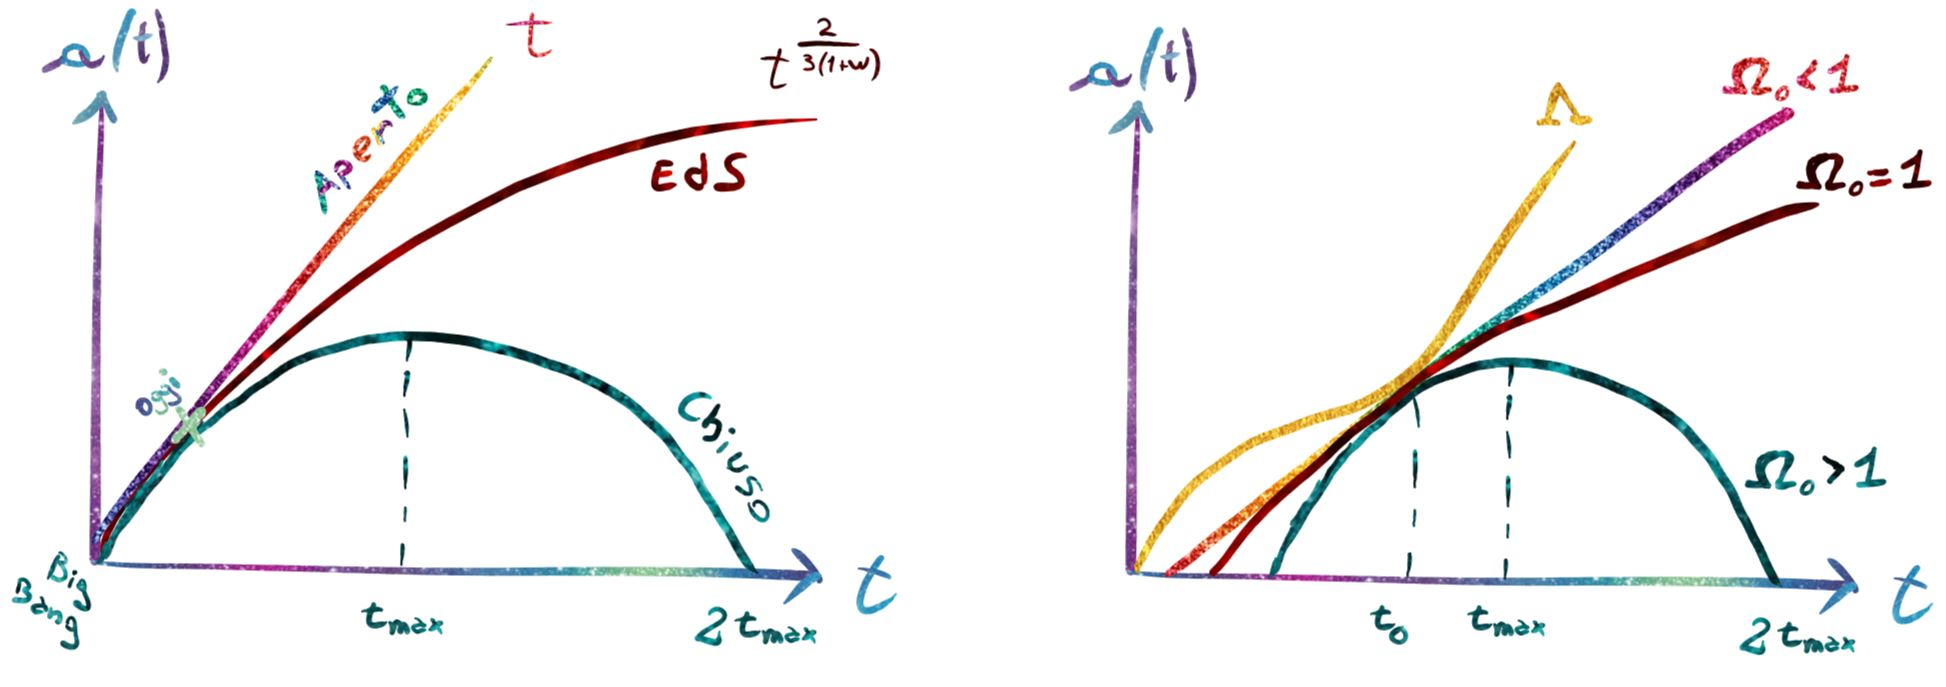
\includegraphics[width=.95\textwidth]{Pictures/2/modellia-t.jpg}
    \caption{Andamento di $a$ al variare del tempo per universi di Friedmann con differenti geometrie. Tutti e tre sono vincolati ad avere un Big Bang per le assunzioni del modello. Il valore $t_0$ si pone prima del massimo dato che si osserva $\dot{a}>0$. Attenzione, il grafico di sinistra è normalizzato al tempo del Big Bang, quello di destra a oggi e riporta anche l'andamento del modello $\Lambda$CDM.}
    \label{fig:2at}
\end{figure}

Le soluzioni analitiche  si ricavano soltanto per il modello Einstein De Sitter, ma nel caso di universi curvi si possono trovare delle soluzioni in forma parametrica, ossia sfruttando la relazione: 
$$
\left\{\begin{matrix}
y= f(y')\\ 
y'=p
\end{matrix}\right. \qquad \Leftrightarrow \qquad 
\left\{\begin{matrix}
x= \int \mathrm{d}p \frac{1}{p}\frac{\mathrm{d} f}{\mathrm{d} p}\\ 
y=f(p)
\end{matrix}\right.
$$
Non si troverà quindi il legame formale tra $y$ e $x$, ma saranno entrambi scritti in funzione di un terzo parametro $p$. Nel nostro linguaggio $x$ sarà il tempo e $y$ il fattore di scala, quindi la relazione tra $a$ e $t$ si studierà attraverso un terzo parametro.

\subsection{Universi di sola materia}
Si assume $c=1$ e $w=0$, ossia \textbf{universi di materia} (di polvere) e si sostituisce la relazione (\ref{eq:rhoaw}) nella seconda equazione di Friedmann (\ref{eq:friedmann2}). Definendo il parametro $p:=\dt{a}$ e la costante $A:= 8\pi G ~\rho_0 ~ a_0^3 /3$, si ottiene:
\begin{equation*}\left\{
\def\arraystretch{1.5}
    \begin{array}{ll}
    t=-\int \mathrm{d}p \frac{2A}{(p^2+k)^2} \\
    a=\frac{A}{p^2+k}
\end{array}\right.
\end{equation*}
Nel caso di \textbf{universo chiuso} ($k=+1$) si procede tramite la sostituzione $p= \tan \theta \rightarrow \mathrm{d}p=\mathrm{d}\theta / \cos^2 \theta$ e definendo $2\theta = \pi-\alpha$:
\begin{equation*}\left\{
\def\arraystretch{1.5}
    \begin{array}{ll}
    t=\frac{A}{2}(\alpha - \sin \alpha) \\
    a=\frac{A}{2}(1 - \cos \alpha)
\end{array}\right.
\end{equation*}
Applicando la definizione di $\OmegaO$ e la relazione $a_0^2 ~H_0^2 = (\OmegaO -1)^{-1}$ (dalla \ref{eq:friedmannh0rho0}) si ottengono le soluzioni, che sono tutte le possibili combinazioni della coppia ($a,t$) al variare del parametro $\alpha$:
\begin{equation}\left\{
\def\arraystretch{1.5}
    \begin{array}{ll}
    a=\frac{a_0}{2} \frac{\OmegaO}{\OmegaO -1}    (1 - \cos \alpha) \\
    t=\frac{1}{2H_0} \frac{\OmegaO}{(\OmegaO -1)^{3/2}}  (\alpha - \sin \alpha)
\end{array}\right.
\end{equation}
Si ha $\dt{a}>0$ per $0<\alpha < \pi$, dopodiché la curva si richiude simmetricamente. L'età dell'universo prevista per questo modello è:
\begin{equation*}
    t_0 = \frac{1}{2H_0}\frac{\OmegaO}{(\OmegaO -1)^{3/2}}\left ( \arccos{\left ( \frac{2-\OmegaO}{\OmegaO} \right )}  -\frac{2}{\OmegaO}\sqrt{\OmegaO-1} \right )
\end{equation*}
Si può verificare che questa età è sempre minore rispetto a quella dell'universo EdS (a parità di $H_0$):
\begin{equation}
t_0 = \mathfrak{C} \frac{1}{H_0}\qquad \mathfrak{C}< 2/3
\end{equation}

\vspace{1em}
In modo analogo è possibile trovare le soluzioni parametriche nel caso di \textbf{universo aperto} ($k=-1$) di sola materia: 
\begin{equation}\left\{
\def\arraystretch{1.5}
    \begin{array}{ll}
    a=\frac{a_0}{2} \frac{\OmegaO}{1-\OmegaO}    (\cosh \alpha -1) \\
    t=\frac{1}{2H_0} \frac{\OmegaO}{(\OmegaO -1)^{3/2}}  (\sinh \alpha -\alpha)
\end{array}\right.
\end{equation}
\begin{equation}
t_0 = \mathfrak{C} \frac{1}{H_0}\qquad \mathfrak{C}> 2/3
\end{equation}
Da queste relazioni si ha un'espansione infinita con un comportamento asintotico $a\propto t $ (come già osservato in precedenza).

\vspace{1em}
\noindent Tutte le soluzioni analitiche ricavate in questo paragrafo, esplicite o parametriche, valgono soltanto nel caso in cui si considera un universo a un'unica componente. Per studiare l'effetto di più componenti le equazioni rimangono sotto forma di integrali e vanno risolte numericamente.

Sommario («Ok quello che stiamo facendo?»):
\begin{itemize}
    \item Soluzioni dei modelli di Friedmann per una sola componente;
    \item Soluzioni analitiche esplicite per EdS;
    \item Soluzioni parametriche per universi curvi di sola materia.
\end{itemize}

\subsection{Proprietà generali}
Utilizzando la relazione $\dt{a}= a ~H_0 ~E$ nell'equazione (\ref{eq1:mathfrankf}):
\begin{equation}
    \mathfrak{f}(r) = \int_{a}^{a_0} \frac{c ~\mathrm{d}a'}{a' ~\dt{a}'} = \frac{c}{H_0} \int_{a}^{a_0} \frac{\mathrm{d}a'}{E ~a'^2}
\end{equation}
Nel caso di universo piatto ($\OmegaTOT=1$), si ha $\mathfrak{f}(r)=r$ e la distanza angolare vale:
\begin{equation}
    d_A = \frac{c}{H_0 (1+z)} \int^z_0 \frac{\mathrm{d}z}{E(z)} 
\end{equation}
negli altri casi è necessario applicare un arcoseno o un arcoseno iperbolico a $r$. 
A questo punto ``si fa partire il cronometro'', ossia si studia il legame tra tempo e redshift. Dalla (\ref{eq:hevol}) per la \textbf{sola materia}, $w=0$, si ha:
\begin{equation}
\dt{a}=a_0~H_0~\sqrt{1+ \OmegaO \:z} \label{eq:adotsolamateria}
\end{equation}
Tramite la relazione $1+z=a_0/a$ si ottiene il legame differenziale tra $t$ e $z$ e integrando:
\begin{align}
    t(z) &=\int_z^\infty \frac{1}{H_0}(1+z')^{-2}(\OmegaO z'+1)^{-1/2}\mathrm{d}z' \\
    & \approx  \frac{1}{H_0 \sqrt{\OmegaO}}~\frac{2}{3} z^{-3/2} \qquad per\quad \OmegaO\: z \gg 1
\end{align}
Siamo felici perché vicino al Big Bang (curvatura ininfluente) ritroviamo la dipendenza prevista dal modello EdS. Per più di una componente bisogna integrare la formula generale:
\begin{equation}
    \mathrm{d}t = - \frac{1}{H_0 ~E(z)}\frac{1}{(1+z)}\mathrm{d}z \qquad\qquad e.g. \quad E(z) = \Omegamo(1+z)^3 + \OmegaLo
\end{equation}
La quantità ``complementare'' all'età dell'universo oggi è il \textbf{Lookback Time} (individua la distanza temporale di un evento a $z$ rispetto a noi osservatori):
$$
t_{LB}(z) = t_0 - t(z)
$$

Sia la densità, sia la densità critica possono dipendere dal tempo, a maggior ragione anche $\Omega$ non sarà costante nel tempo. Dalle equazioni (\ref{eq:rhoaw}) e (\ref{eq:hevol}) si può calcolare:
\begin{equation*}
    \Omega(z) = \frac{\rho(t)}{\rho_{cr}(t)} \qquad\rightarrow \qquad \Omega^{-1}(z) -1 = \frac{\OmegaO^{-1}-1}{(1+z)^{1+3w}}
\end{equation*}
che misura quanto dista dall'unità $\Omega (z)$ rispetto a quanto dista dall'unità oggi. Se oggi $\OmegaO$ vale 1 (universo piatto), $\Omega(t)$ sarà sempre stato e sempre sarà 1. Se $\OmegaO > 1$, allora $\Omega(z) > 1\;  \forall z$ e se $\OmegaO < 1$, allora $\Omega(z) < 1\;\forall z$. L'universo non può cambiare la sua geometria durante la sua evoluzione.
\begin{figure}[ht]
    \centering
    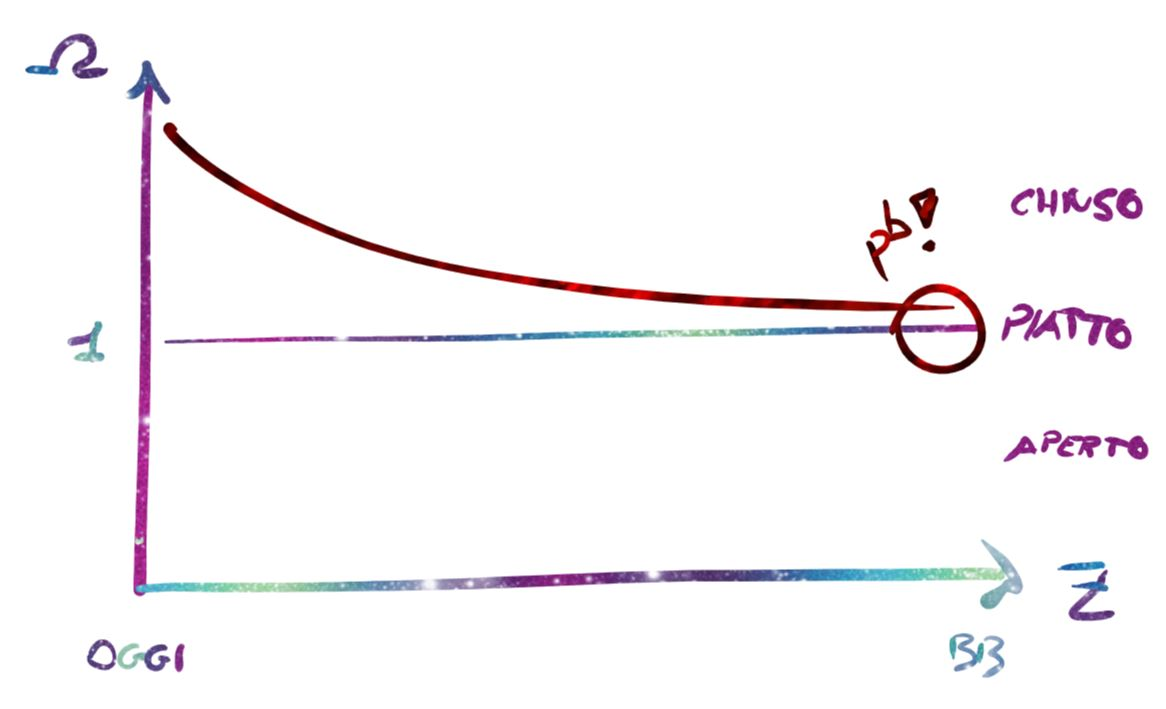
\includegraphics[width=.8\textwidth]{Pictures/2/omega-z.jpg}
    \caption{Problema della piattezza. Aver osservato $\OmegaO = 1$ richiede un immenso fine-tuning di $\Omega_{BB}$ per questo modello.}
    \label{fig:2omegaz}
\end{figure}

Se si ha più di una componente, la formula generale da utilizzare è:
\begin{equation}
    \Omega (z) = \OmegaO \frac{(1+z)^{3(1+w)}}{E(z)^2}
\end{equation}


\begin{definition}[Problema della Piattezza]
 Oggi si misura $\OmegaO =1$ (e già negli anni `70 si sapeva che $\OmegaO \approx 1$). Ma dal Big Bang è passato talmente tanto tempo che, per avere oggi questo valore, doveva inizialmente valere $1$ con una precisione di $10^{-60}$ (valore estremamente preciso da essere innaturale). 
\end{definition}


\section{Orizzonte cosmologico}
Ci si aspetterebbe che l'universo in connessione causale con noi osservatori sia $c\, \Delta t$, ma l'universo si espande! Si definisce quindi il \textit{raggio dell'orizzonte cosmologico (o delle particelle)} la quantità:
\begin{equation}
    R_H (t) = a(t) \int_0^t \frac{c\, \mathrm{d}t'}{a(t')} \label{eq:raggioriz}
\end{equation}
che stabilisce la massima distanza comovente da cui la luce prodotta in passato può aver raggiunto l'osservatore.

Per $a \rightarrow 0$ quando $ t \rightarrow 0$ pare accadere che $R_H \rightarrow \infty$. Implicherebbe che tutto l'universo al Big Bang fosse in connessione causale (che senso avrebbe definire un raggio?), ma questo non succede. Si può infatti verificare che quando il termine di curvatura è trascurabile:
\begin{equation*}
    R_H (a) = a(t) \int_0^{a(t)} \frac{c\, \mathrm{d}a'}{a' \: \dt{a}'} \quad = \frac{2}{1+3w} \frac{c}{H_0\, \OmegaO^{1/2}} \left ( \frac{a}{a_0} \right)^{\frac{3(1+w)}{2}}
\end{equation*}
Quindi il raggio dell'orizzonte per $a \rightarrow 0$ non diverge. Si utilizzerà una sola componente, infatti come verrà discusso a breve vicino al Big Bang domina soltanto quella radiativa. In ogni caso, per un universo EdS si avrebbe:
\begin{equation}
    R_H (t) = \frac{2}{1+3w}\frac{c}{H_0}\frac{t}{t_0} = 3ct \left ( \frac{1+w}{ 1+3w} \right )= \left\{\begin{matrix}
3ct & w=0\\ 
2ct & w=\frac{1}{3}\: (BB)
\end{matrix}\right.
\end{equation}
Quindi cresce più velocemente di $ct$, ossia mette in comunicazione regioni più vaste di quanto ci si aspettava. $R_H$ rappresenta la scala su cui bisogna considerare le interazioni causali (microfisica), al suo esterno agisce solo la gravità.

Un altro modo per definire l'orizzonte è la \textbf{Sfera di Hubble} (o raggio dell'orizzonte effettivo), definita come la distanza che ha un oggetto che si sta muovendo nel flusso di Hubble con velocità $c$. Oppure, analogamente, la distanza che percorre la luce in un'unità di tempo tipica del tempo di espansione dell'universo ($1/H$): 
\begin{equation}
    \tilde{R}_H (t) = c\: \tau_{exp} = \frac{c}{H}
\end{equation}
Mentre la definizione precedente era una quantità integrale sulla sfera di espansione temporale, in questo caso si ha un valore istantaneo definito da $H(t)$. Per l'universo primordiale vale $R_H \equiv \tilde{R}_H (t)$. Nel caso di universi EdS si ha:
\begin{equation*}
    \tilde{R}_H (t) =  \frac{1+3w}{2} R_H
\end{equation*}
Il tempo tipico di espansione è fondamentale per decidere quali processi, in determinati periodi della storia dell'universo, possono essere considerati trascurabili o meno.

Si definisce invece \textit{raggio dell'orizzonte degli eventi} la quantità:
\begin{equation}
     R_E (t) = a(t) \int_t^\infty \frac{c\, \mathrm{d}t'}{a(t')}
\end{equation}
che stabilisce la massima distanza comovente da cui la luce prodotta a $t$ potrà mai raggiungere l'osservatore. Questa quantità non è solitamente utilizzata in cosmologia e non esiste per modelli di Friedmann con $-1/3<w<1$ (ma esiste nel modello di De Sitter). Tutti i modelli di Friedmann prevedono invece un Big Bang e un orizzonte cosmologico finito. 

\section{Componenti osservate nell'universo}

\subsubsection{Galassie}
La funzione di luminosità di Schechter provvede una descrizione parametrica della densità spaziale delle galassie in funzione della loro luminosità:
$$
\phi (L) = \frac{\phi_*}{L_*} \left ( \frac{L}{L_*}  \right)^{-\alpha}e^{-L/L_*}\qquad \mathcal{L}_{tot}=\int \phi (L) \, L \, \mathrm{d}L
$$
Mediante una stima del rapporto $M/L$ di ottiene una stima di $\rho_{gal} \simeq 0.02\: \rho_{\mathrm{cr},0}$ riferita alle galassie luminose.
\begin{equation}
    \Omega_{gal}=0.02
\end{equation}

\subsubsection{Materia Barionica}
Esiste inoltre materia barionica che non è nelle galassie (e non produce sufficiente luce). Si può ottenere una stima di questo contributo tramite due approcci diversi. Uno è il modello della nucleosintesi primordiale, necessario per spiegare le abbondanze degli elementi leggeri che si osservano oggi. Il secondo sfrutta la fluttuazione delle buche di potenziale osservabili dalla CMB ed è più preciso.
\begin{equation}
    \Omegab=0.04 \div 0.05
\end{equation}

\subsubsection{Materia Oscura}
Osservabile indirettamente grazie agli effetti gravitazionali: dinamica di galassie e ammassi, lensing gravitazionale, CMB, LSS. Tutti i diversi approcci danno un valore abbastanza consistente della densità della materia oscura.
\begin{equation}
    \OmegaDM=0.25 \div 0.26
\end{equation}

Ai fini cosmologici le tre componenti appena viste hanno $w=0$ e si possono buttare nel mucchio di tutta la materia:
\begin{equation}
    \Omegam= 0.3
\end{equation}

\subsubsection{Radiazione}
A quanto pare sappiamo chiamare ogni fotone per nome, uno ad uno. I fotoni della CMB sono prodotti in una situazione di equilibrio, per questo motivo sono distribuiti come un corpo nero. Misurando la temperatura della radiazione oggi ($T_{r\, 0}=2.726$ K), si può calcolare la loro densità oggi ($\rho_r c^2 = \sigma T_r^4$), che risulta essere $\rho_r=4.8\cdot 10^{-34}$ g cm$^{-3}$.
\begin{equation}
    \Omegar h^2\simeq 2.5\cdot 10^{-5}\approx 0
\end{equation}
(Tutti gli altri fotoni prodotti da stelle, ... sono trascurabili rispetto alla marea di fotoni della CMB).

\subsubsection{Neutrini et al.}
Se i neutrini non hanno massa, sono relativistici e anche per loro vale la relazione $\rho_\nu c^2 = \sigma T_\nu^4$. Per un valore stimato di $T_{\nu 0}=1.9$ K si avrebbe una densità ancora più piccola rispetto a quella della radiazione, circa il 70\%. Se avesse massa non si include nel contributo della radiazione, ma in quello della DM (a ritroso, conoscendo $\OmegaDM$, si può stimare la massa del neutrino).

\subsubsection{Dark Energy}
Tramite evidenze osservative (scala dell'orizzonte cosmologico al momento della CMB) si sa che $\OmegaTOT=1$.
Il contributo della costante cosmologica è dedotto per sottrazione:
\begin{equation}
    \OmegaLo = 1 - \sum \Omega_{i\: 0}
\end{equation}

Un modo diverso per ottenere il suo contributo è tramite l'osservazione dell'espansione accelerata dell'universo (SNe): $q \approx -0.5$. Utilizzando la prima equazione di Friedmann e la definizione di $q$, si ottiene per universi di sola materia ($p=0$):
$$
q = \frac{\Omegam}{2}\approx 0.15
$$
a differenza di quanto osservato, per cui è necessaria una componente aggiuntiva, che nel caso di $\Lambda$ porta a:
$$
q = \frac{\Omegam}{2} -\OmegaL \equiv -0.5 \qquad\rightarrow\qquad \OmegaL \approx 0.7
$$
Si è già calcolato che, per avere accelerazione positiva nelle equazioni di Friedmann, deve valere la condizione $w< -1/3$ che caratterizza la \textit{dark energy}. Il caso particolare in cui $w=-1$ ad ogni $t$ definisce la \textit{costante cosmologica}. Quindi la dark energy è una famiglia larga di modelli che comprende anche quello della costante cosmologica (secondo i dati il più probabile).

\subsubsection{Commenti qualitativi a caldo}
Dalla Fig. \ref{fig:2rhored} e dai valori appena ottenuti si può osservare che:
\begin{itemize}
    \item Esistono due periodi di equivalenza: materia-radiazione e materia-$\Lambda$;
    \item Soltanto oggi domina la costante cosmologica (\textbf{problema della coincidenza});
    \item La radiazione domina soltanto nella prima epoca dell'universo.
    \item Nel periodo intermedio possiamo considerare l'universo composto solo da materia.
\end{itemize}

Utilizzando la relazione (\ref{eq:rhoaw}) è possibile calcolare una stima per il redshift a cui si hanno le due equivalenze:
\begin{align}
  & z_{eq,\, rad}=\frac{0.3}{2.6\cdot 10^{-5}h^2} \simeq 5000  \\
  & z_{eq,\, \Lambda}= \left ( \frac{\OmegaLo}{\Omegamo} \right) ^{1/3} -1 \simeq 0.3  
\end{align}
Dato che un'eventuale curvatura, se esiste, si percepisce per $z<1/\OmegaO$, le considerazioni appena fatte (valevoli per un'universo EdS) sono una buona approssimazione nel nostro universo.

In aggiunta alla Fig. \ref{fig:2at} si può calcolare l'andamento di $a(t)$ per oggi, ossia nell'unico periodo della storia dell'universo in cui domina $\Lambda$. Ci si aspetta un'accelerazione, quindi un flesso ad un certo $t$ dal quale la curva si allontana dal modello EdS:
\begin{equation}
    z_{flex,\, \Lambda}= \left ( \frac{2 \OmegaLo}{\Omegamo} \right) ^{1/3} -1 \simeq 0.6 
\end{equation}
Questo valore è alla base del \textbf{problema della coincidenza} che verrà discusso a breve.

In conclusione si riporta un andamento dei vari parametri cosmologici al variare del tempo, quindi del parametro $a$ (Fig. \ref{fig:2omeghe}) e un' illustrazione di tre diversi modelli cosmologici (Fig. \ref{fig:2geom}).

\vspace{1em}
\begin{figure}[H]
    \centering
    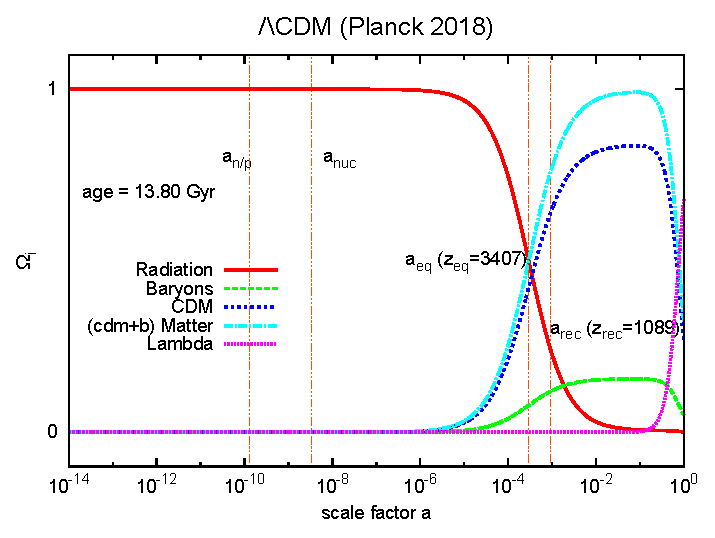
\includegraphics[width=.85\textwidth]{Pictures/2/densparplank.eps}
    \caption{Evoluzione dei parametri di densità delle varie componenti modellate utilizzando una cosmologia $\Lambda$CDM e i dati di Planck (From: \cite{rindlerdaller2019understanding}).}
    \label{fig:2omeghe}
\end{figure}


\begin{figure}[ht]
    \centering
    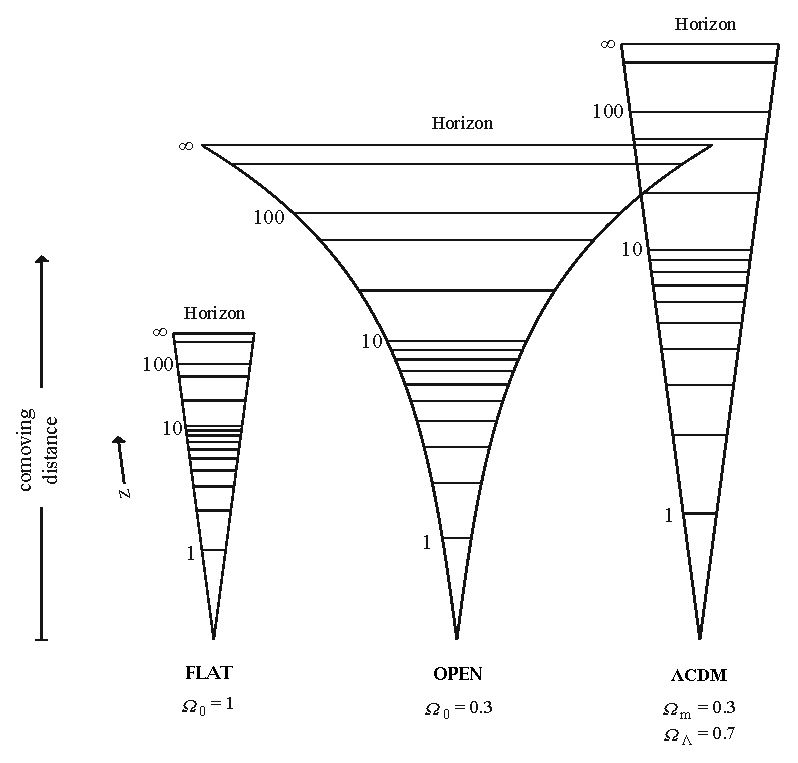
\includegraphics[width=.95\textwidth]{Pictures/2/geometry.eps}
    \caption{Comportamento dei diametri angolari e delle distanze in funzione del redshift per tre diversi modelli cosmologici: universo piatto, chiuso e $\Lambda$CDM. Ogni spicchio rappresenza un cono di angolo fissato in corrispondenza dell'osservatore. Sono riportate le dimensioni comoventi (lungo la linea di vista e proiettate nel cielo) al variare delle quantità osservabili: redshift e separazione angolare (From: \cite{Hamilton_1998}).}
    \label{fig:2geom}
\end{figure}